\newpage
\subsection{Évolution de carte acoustique}

% Explication
Il y a trois versions de carte acoustique. Les cartes de version 4G (V4G) sont déjà en fabrication, la version 0 (V0) est en cours de développement, et la version 1 (V1) est en cours de conception.\\

Voici un schéma pour présenter l'évolution de carte acoustique développée par UINT:

\begin{figure}[!htbp]
  \centering
    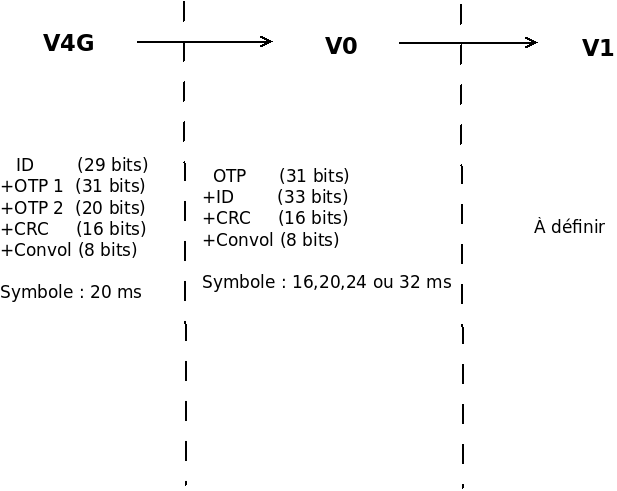
\includegraphics[scale=0.5]{images/version}
  \caption{Évolution de carte acoustique}
  %\label{fig:auth}
\end{figure}

%%%%%%%%%%%%%%%%%%%%%%%%%%%%%%%%%%%%%%%%%%%%%%%%%%%%%%%%%%%%%%%%%%%%%%%%%%%%%%%%%%%
\subsection{Cahier des charges}
\label{CDC}
Comme indiqué dans chapitre \ref{sujet}:Présentation du sujet du stage , mon travail est divisé en deux parties:\\

\begin{itemize}
\item Concevoir les tests pour la version 4G (V4G)
\item Développer d'un site de démonstration pour l'utilisation la carte acoustique
\end{itemize}
%%%%%%%%%%%%%%%%%%%%%%%%%%%%%%%%%%%%%%%%%%%%%%%%%%%%%%%%%%%%%%%%%%%%%%%%%%%%%%%%%%%
\newpage
\subsection{Outils}

Les outils pour réaliser les tâches:

\subsubsection{Offline}

L’utilitaire \texttt{ListenAcousticMessage\_V1.2.1.35.exe}, développé par UINT, permet de voir le message acoustique produit par la carte pour les systèmes sous Windows.

\subsubsection{Online}

La page de test pour Internet Explorer (IE), disponible sous l’url suivante, permet de voir le message acoustique produit par la carte: 

\url{http://solution.uint.info/AcousticMessage}

\subsubsection{Transcodage}

Le transcodage est l’opération de conversion du message acoustique physique, le bruit de la carte, en un message numérique informatique
 
\subsubsection{Décodage}

Le décodage est l’opération de conversion du message transcodé en une structure plus simple présentant les informations individuelles ici le numéro de série et les OTPs. Dans la version 4G de carte les informations sont simplement concaténées.
 
\subsubsection{Authentification}

Un serveur d’authentification est accessible en ligne. Une description est détaillée dans la section \ref{SAS}.


%%%%%%%%%%%%%%%%%%%%%%%%%%%%%%%%%%%%%%%%%%%%%%%%%%%%%%%%%%%%%%%%%%%%%%%%%%%%%%%%%%%
\newpage
\subsection{Architecture globale du système de démonstration} 

Voici une archutecture globale d'un système que l'utilisateur peut s'authentifier avec sa carte acoustique:

\begin{figure}[!htbp]
  \centering
    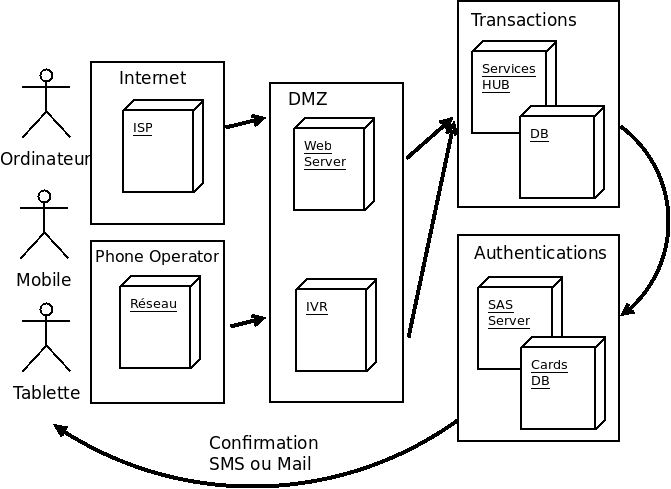
\includegraphics[scale=0.6]{images/arch}
  \caption{Schéma d'architecture globale}
  %\label{fig:auth}
\end{figure}


%L'utilisateur peut utiliser sa carte acoustique comme un moyen d'authentification pour faire un paiement par exemple.\\

Le système est divisé en 6 parites:
\begin{itemize}
\item ISP
\item Opérateur téléphonique
\item IVR
\item Serveur Web
\item Base de données 
\item Serveur d'authentification\\
\end{itemize}


Comme nous avons besoin d'utiliser la carte acoustique dans l'environnement téléphonique, on a besoin d'un opérateur téléphonique, et aussi, un SVI.



